\section{Inference Methodology}

%For the SEI:

%Census data + geolocalization + ARPU + cellphone payments (recharges)  --> SEI estimation for geolocalized users. 

%Second, we extended our predictions taking advantage of graph structure and socioeconomic homophily. To this end, we considered a bayesian  

%\sout{As part of the dataset from the bank \( B \), we have the monthly salaries of most bank users \( B_{S_0} \cdots B_{S_t} \) for a period \( t \) larger than \( M \). We considered the average of \( B_{S_i} \) for a period of \( 6 \) moths to generate \( B_S \)}

%\sout{To infer the monthly salary of the users we take the average of \( B_{S_i} \) for a period of \( 6 \) moths to generate \( B_S \), and we compare them with other users' salaries by using the link correlations in \( G_N \).}

The main contribution of this work is the estimation of the income of the telco users for which we lack banking data but have bank clients in their neighborhood of network graph. To show the feasibility of this task we first show the existence of a strong income homophily in the telco graph as is evidenced in Figure x.

For each pair \( \left< o, d \right> \in \mathlarger{G} \) we define \( X \) as the set of incomes for callers and \( Y \) as the set of incomes for callees. According to what we can observe in Figure x, \( X \) and \( Y \) should be significantly correlated. Given the broad non gaussian distribution of the income's values, we choose to use a rank based measure of correlation, namely the \textbf{Spearman's rank correlation} to test the statistical dependence of sets \( X \) and \( Y \) using the following formula: 

\[
r_s = \mathlarger{\rho}_{\operatorname{rank}(X) \operatorname{rank}(Y)} = \frac{\operatorname{cov}(\operatorname{rank}(x), \operatorname{rank}(y))}{\sigma_{\operatorname{rank}(X)} \sigma_{\operatorname{rank}(Y)}}
\]

If we compare our data with a randomized null hypothesis, where links between users are selected randomly disregarding income data, this coefficient gives us a correlation of \num{0.474} with a P-value of $ P < 10^{-6} $. This is significant enough to show that there is a significant amount of homophily between users' incomes in our data.

We can take advantage of this homophily to propagate income information to the rest of our graph $ \mathlarger{P} $, where we don't know the income of all of the users.

To achieve this, we define 2 balanced income categories according to the median of the resulting income distribution: the set $ \mathlarger{G}_W $ of \textbf{Wealthy people}, whose income is on the upper half of the dataset, and the set $ \mathlarger{G}_P $ of \textbf{Poor people}, whose income is on the lower half. We should be able to predict if a used in $ \mathlarger{P} $ is on the upper or lower income category with the information of the links to other users.

\begin{figure}[]
\begin{center}
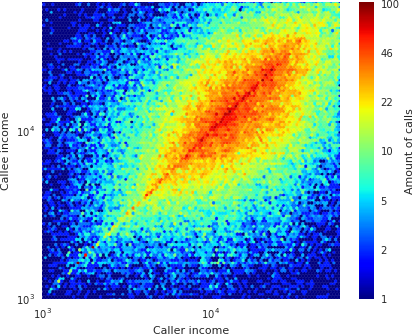
\includegraphics[width=1\columnwidth]{figures/Homophily_income_origin_target_1/Homophily_income_origin_target_1.png}
\caption{ \protectReplace this text with your caption}
\end{center}
\end{figure}

More precisely, we compute for each user $ g \in \mathlarger{G} $, we define its call distribution across the defined income categories as $ \alpha_1 $, the fraction of calls to wealthy users, and $ \alpha_0 $, the fraction of calls to poor users. These calls distributions were used as the parametrization vector of a \textbf{Dirichlet distribution} $D(\alpha_p)$ for each user $ p \in P $. We can interpret the sample space of $ D(\alpha_p) $ as a discrete probability distribution and considering out initial assumption of data homophily homophily, we expect that users belonging to a certain category tend to be concentrated to this particular category.

